\documentclass[a4paper, 12pt]{article}%тип документа

%отступы
\usepackage[left=2cm,right=2cm,top=2cm,bottom=3cm,bindingoffset=0cm]{geometry}

%Русский язык
\usepackage[T2A]{fontenc} %кодировка
\usepackage[utf8]{inputenc} %кодировка исходного кода

%Вставка картинок
\usepackage{wrapfig}
\usepackage{graphicx}
\graphicspath{{pictures/}}
\DeclareGraphicsExtensions{.pdf,.png,.jpg}

%Графики
\usepackage{multirow}
\usepackage{pgfplots}
\pgfplotsset{compat=1.9}

%Математика
\usepackage{amsmath, amsfonts, amssymb, amsthm, mathtools}

%Заголовок
\author{Hasib Sifat and Vladimir Shmakov \\
Faculty of Physical and Quantum Electronics \\
GROUP Б04-105}
\title{\textbf{LABORATORY WORK 3.1.1 \\ 
Magnetometer}}
\begin{document}
\maketitle

\begin{abstract}
Using some simple equipment we have calculated the horizontal component of the Earth's magnetic field with $84.4 \%$ accuracy and establish a quantitative relationship between the units of the electric current in SI and CGS systems and find almost the accurate value of the speed of light.
\end{abstract}

\section{Introduction} A magnetometer is a device for magnetic measurements, for example: compass, theodolite, webermeter, etc. With the help of magnetometers, the magnetization of ferromagnets, the intensity of magnetic fields, investigate magnetic anomalies. Magnetometers
of various designs have been developed: magnetostatic, electromagnetic, magneto-dynamic, induction, resonant. Reference magnetometers they allow measuring the horizontal and vertical components of the intensity of the Earth's magnetic field with an accuracy of $10^{-6}$ E. In our installation using an electromagnetic magnetometer from the horizontal component of the earth's magnetic field is measured and the current strength is determined by its magnetic action in an absolute way.

\textbf{Equipment we used:} Magnetometer, illuminator with scale,
power source, voltmeter, electromagnetic switch, capacitor, magnetized rod, device for determining the period of torsional oscillations, stopwatch, tape measure, caliper.
 

\section{Experimental Setup:} The magnetometer (Fig. 1) consists of several sequentially connected circular coils K, arranged vertically. In the center of the ring with radius R, a short magnetic arrow C is suspended on a thin inelastic vertical thread. The impeller rigidly connected to the arrow is immersed in oil and serves to dampen vibrations.\\
\begin{figure}[h]
\begin{center}
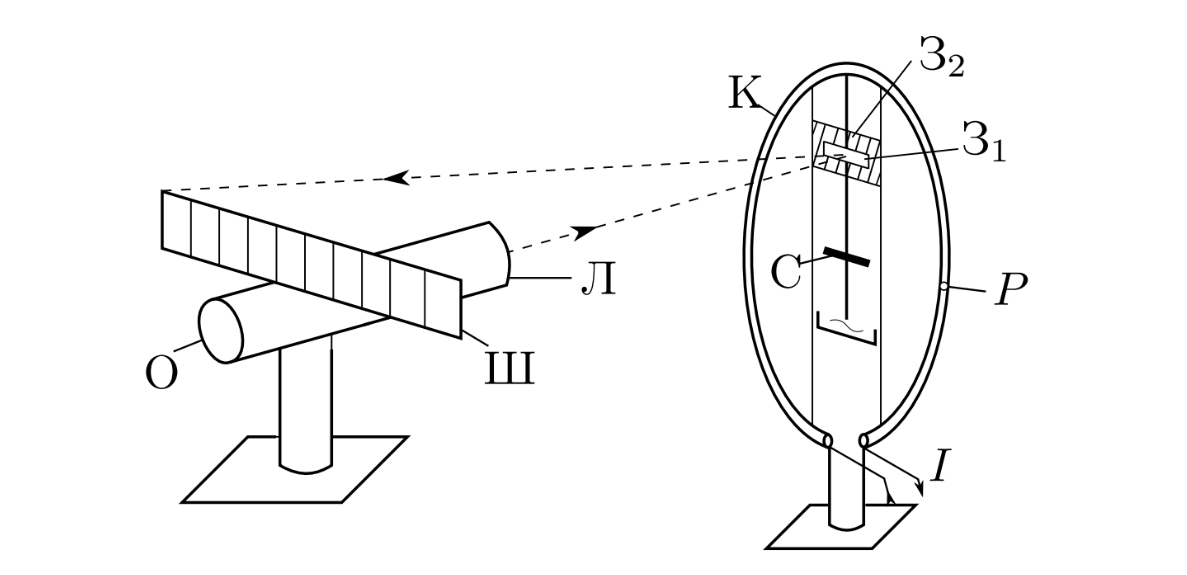
\includegraphics[width = 0.8\textwidth]{Fig1.png}
\caption{Magnetometer diagram}
\end{center}
\end{figure}

\begin{figure}[h]
\begin{center}
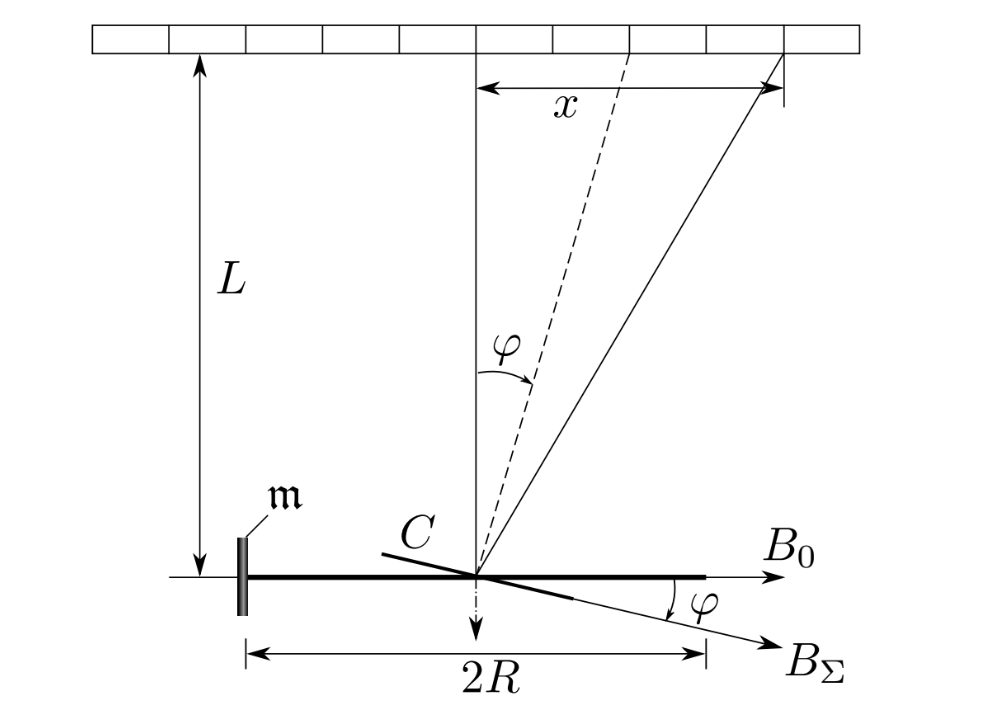
\includegraphics[width = 0.8\textwidth]{Fig2.png}
\caption{The scheme of measuring the angle of deviation of the magnetic needle}
\end{center}
\end{figure}
In the absence of other magnetic fields, the arrow is located along the
direction of the horizontal component of the earth's magnetic field \textbf{$B_0$},that is, it lies in the plane of the magnetic meridian. The device is adjusted with the help of light bunnies reflected from two mirrors: $Z_1$, attached to the arrow (movable bunny), and $Z_2$ is located in the plane of the ring K and rigidly connected to it (not a moving bunny). Both mirrors are illuminated by the same illuminator O. By rotating the ring around the vertical axis, it is possible to combine both bunnies. In this case, the plane of the turns coincides with the plane of the magnetic meridian.\\
\newline
When an additional horizontal magnetic field \textbf{$B_{\perp}$} appears, the arrow C will be set according to the resultant of both fields \textbf{$B_{\sum}$} (Fig. 2). In our installation, an additional field can be created either by a small ferromagnetic rod located on the ring at its horizontal diameter \textbf{$B_1$}, or by a current passing through the ring \textbf{$B_2$}. In both cases, the additional field can be considered homogeneous, since the dimensions of the arrow are much smaller than the radius of the ring. The field of a magnetized rod away from it can be approximately calculated as the field of a point dipole:

\begin{center}
$\textbf{B(r)} = \frac{\mu_0}{4\pi}(3\frac{(\textbf{m}.r).r}{r^5}-\frac{\textbf{m}}{r^3}) $
\end{center}
where \textbf{m} is the magnetic moment of the rod, r is the radius vector drawn from the center of the dipole to the observation point. On the axis perpendicular to the rod, we have
\begin{center}
$\textbf{B(r)} = \frac{\mu_o}{4\pi}\frac{\textbf{m}}{R^3}$.......(1)
\end{center}
where R is the radius of the ring.\\
\newline
The magnetic field in the center of the ring with current I according to the Biot–Savart law is equal to:
\begin{center}
$B = \frac{\mu_0I}{2R}N$.......(2)
\end{center}
Here N is the number of turns in the ring, I is the current strength in SI units (ampere).\\
\newline
By measuring the angle of deviation of the arrow $\varphi$, we can connect the fields $B_0$ and $B_{\perp}$($B_1$ or $B_2$):
\begin{center}
$B_{\perp}=B_0 \cdot tg\varphi$.......(3)
\end{center}
\textbf{Determination of the Horizontal Component Earth's Magnetic Field}:\\
\newline
To determine the horizontal component of the Earth's magnetic field $B_0$, a thin short magnetized rod is installed in the hole P on the horizontal diameter of the ring (Fig. 1). Measuring the tangent of the angle of deviation of the arrow:
\begin{center}
$tg\varphi_1=\frac{x_1}{2L}$.......(3)
\end{center}
it is possible to calculate the field $B_0$ using equations (1),(3) and (4), if we exclude the value \textbf{m} — the magnetic moment of the rod. To exclude the magnetic moment, it is proposed to measure the period of torsional vibrations of the rod in the Earth's field. Suspended horizontally by the middle on a thin long thread, the rod is in position the equilibrium will be established along the Earth's field (the elasticity of the thread is negligible). If the axis of the rod is deflected in the horizontal plane from direction $B_0$ at a small angle $\alpha$, then under the action of the returning mechanical moment:
\begin{center}
$ M_{mech} = | m \times B| = mB_0sin\alpha \approx mB_0\alpha $
\end{center}
a rod with a moment of inertia J in accordance with the equation:
\begin{center}
$J\ddot{a} + \textbf{m}B_0\alpha = 0$
\end{center}
will make torsional oscillations with a period of

\begin{center}
$T = 2\pi \sqrt{\frac{J}{\textbf{m}B_0}}$.......(5)
\end{center}

The moment of inertia of the cylindrical rod relative to the axis
of rotation:
\begin{center}
$J= m(\frac{l^2}{12}+\frac{r^3}{4}) = \frac{ml^2}{12}[1+3(\frac{r}{l})^2]$.......(6)
\end{center}
where m is the mass of the rod, l is the length, and r is its radius.\\
\newline
Thus, by calculating the moment of inertia J and measuring the tangent of the angle of deviation of the arrow $\varphi_1$ and the period of small torsional vibrations of the rod T, it is possible using the formulas (1), (3), (4) and (5) determine the horizontal component of the Earth's magnetic field:

\begin{center}
$B_0 = \frac{2\pi}{TR}\sqrt{\frac{\mu_0JL}{2\pi Rx_1}}$ [SI].......(7)
\end{center}

Since the magnetometer is installed in a reinforced concrete building, the magnetic field in it can not only differ greatly from the Earth's field, but also vary markedly from place to place, so the oscillation period should be measured directly near the magnetometer. In addition, in order to ensure maximum uniformity of the magnetic field in the measurement area, powerful sources of a strong magnetic field should be eliminated (removed to the maximum distance): power sources, current-carrying wires, cell phones, metal objects, etc.\\
\newline
\textbf{Determination of the Electrodynamic Constant (The Speed of Light):}\\

The current in the ring circuit can be measured in two independent ways: by the magnetic action of the current on the magnetometer needle and by the charge flowing through the circuit per unit of time. The first method of measurement corresponds to how the current standard is defined in the SI system, and the second — in the Gaussian system (CGS). With respect to the results of these measurements, the electrodynamic constant c can be determined. Passing some current through the coils of the magnetometer, we measure the tangent of the angle of deviation of the arrow ($tg\varphi = x_2/2L$)and calculate the current strength using formulas (2) and(3):
\begin{center}
$I = \frac{2B_0R}{\mu N}tg\varphi_2$ [SI]........(8)
\end{center}
The value $A = 2B_0R/(\mu_0N)$ is the constant of the device in a given place of the earth's surface (more precisely, in a given place of the room - taking into account numerous third-party sources of magnetic field). The same current can be measured in an absolute way by the past per unit of time to the charge, which corresponds to the definition of the standard
as in the Gaussian system (CGS). If the capacitor is discharged , capacitance C, charged to voltage U, through the turns, then a charge q = CU will flow through them (Fig. 3). If the capacitor is sequentially
charged from the source once per second and discharged through the turns, then through they will leak a CUv charge in a second.The average current passed through the turns is equal to:
\begin{center}
I = CUv .......(9)
\end{center}

\begin{figure}[h]
\begin{center}
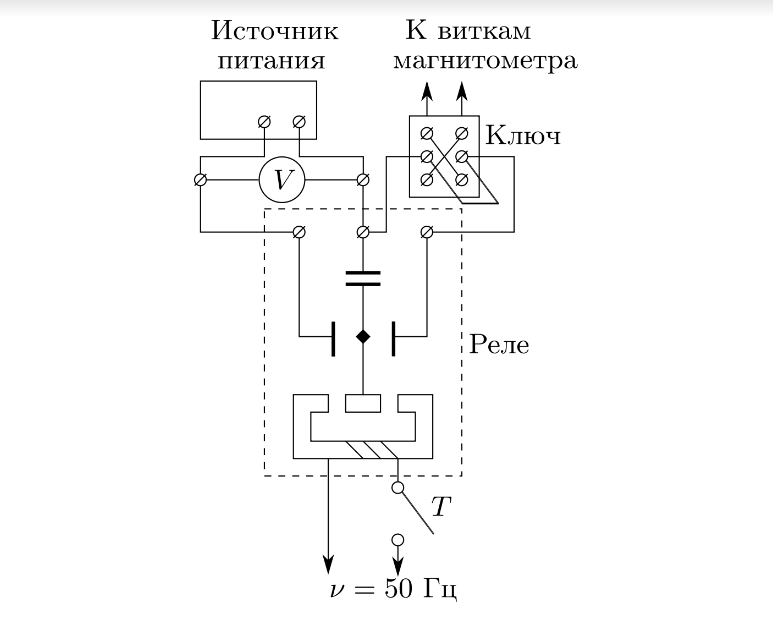
\includegraphics[width = 0.8\textwidth]{Fig3.png}
\caption{The power supply circuit of the magnetometer coil}
\end{center}
\end{figure}
Thus, the absolute measurement of the current is reduced to finding the values of C and G, which can also be determined in an absolute way. So, the capacitance of a flat capacitor can be calculated from its dimensions, that is, relying only on the unit length. The potential difference can also be determined in an absolute way, for example, through the force acting on the plate of a charged capacitor, as is done in an absolute voltmeter (see Work 3.1.2). However, we will not fully carry out this program, but will limit ourselves only to indicating the possibility of its implementation.\\
So, to calculate the absolute value of the current according to (9), it is necessary to measure the voltage U on a capacitor of known capacitance C. The voltage must be expressed in CGS units (measuring instruments are usually graded in SI units: $1V \approx \frac{1}{300}$ units CGS). The capacitance of the capacitor C [cm] should be expressed in centimeters ($1F \approx$ $9 \times 10^{11}$ cm).\\
With respect to the numerical values of the same current, expressed in SI and CGS units (Gaussian) according to formulas (8) and (9), respectively, it is possible to determine the value of the electrodynamic constant:


\begin{center}
$c[\frac{m}{c}]= \frac{1}{10}\frac{I_{[CGS]}}{I_{[SI]}}$........(10)
\end{center}

We suggest that the independently obtain the ratio (10), proceeding from the definition of the ampere and the absolute (Gaussian) unit of current.

\section{Experimental Results and Analysis}
In this work, we have total two tasks. First of all measurement of the horizontal component of Earth's magnetic field and estimating the electrodynamics constant.\\
\newline
\textbf{Measurement of the Horizontal Component of Earth's Magnetic Field}
In the theoretical part we have already explained all the formula that we're gonna use. From our observation, we got

\begin{center}
The oscillation period of the rod is, T = 7.5 $\pm$ 0.4 s\\
Radius of the ring, R = 17 cm\\
Distance from the scale to mirror is, L = 86 cm\\
Length of the cylindrical rod is, l = 4 cm\\
Radius of the cylindrical rod is, r = 0.5 cm\\
Mass of the cylindrical rod is, m = 5.90 g\\
\end{center}
Now using the formula (6), we get the the moment of inertia of the cylindrical rod:

\begin{center}
J = 8.24 $\pm$ 0.05 $g/cm^2$
\end{center}
Now using the formula (7) we get the horizontal component of Earth's magnetic field:

\begin{center}
\framebox{$B_0 = 12668.35 \pm 1119.18 \ nT \approx 13000 \pm 1000 \ nT $}
\end{center}

Now let's compare our result with the real value. To get the real value of the horizontal component of Earth's magnetic field we use  \textbf{International Geomagnetic Reference Field (IGRF), 13th Generation Calculator}. Putting the geographic coordinates of our lab and the date of our experiment, we get the real horizontal component.  
\begin{figure}[h]
\begin{center}
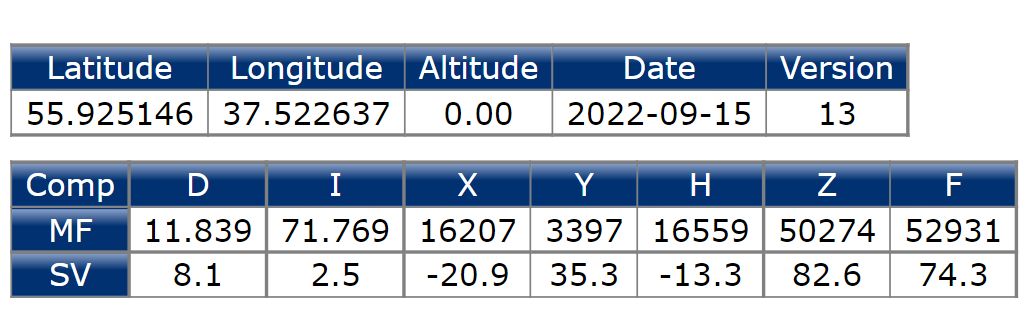
\includegraphics[width = 0.8\textwidth]{Fig4.png}
\caption{Components of Earth's magnetic field in Dolgoprudny on 15th September 2022 }
\end{center}
\end{figure}

We see that the horizontal component on that day is \textbf{16559 nT} and our the result we got is 13000 nT. The deviation is $15.6\%$. So the accuracy in our measurement is \framebox{$84.4\%$}.\\
\newline
\textbf{Measurement of the Electrodynamic Constant (Speed of Light)}:
Now we calculate the current in the direction of the deflection of the magnetic arrow in the field of circular current and the known field of the Earth. We calculate the current in both SI and CGS unit and then using them calculate the speed of light.\\
\newline
Due to the current flow in the ring, we noticed the deflection of the magnetic arrow. Due to the current flow in different direction, we noticed the deviation on the scale is $x_1 = 11.5$ and $x_2 = 12 cm$. By combining them we get the final deviation with error is \framebox{$L = 11.7 \pm 0.5 cm$} \\
\newline 
Now using the formula (8), we find the current strength in SI unit with error:
\begin{center}
\framebox{$I_{SI} = 0.0051 \pm 0.0005 A$}
\end{center}
Now using the formula (9), we can find the current strength in CGS unit with error:
\begin{center}
\framebox{$I_{CGS} = (143 \pm 3) \times 10^5$} CGS unit for current measurement.
\end{center}

Now formula (10) suggests us the electrodynamic constant or the speed of light:
\begin{center}
$c[\frac{m}{c}]= \frac{1}{10}\frac{0.0051 \pm 0.0005}{(143 \pm 3) \times 10^5} = 281406490 \pm 26657523 / m/s = (280 \pm 30) \times 10^6  / m/s$
\end{center}
So we measure the speed of light is \framebox{$(280 \pm 30) \times 10^6  / m/s$}. To estimate the accuracy of our result we compare it with the exact value given in Wikipedia. Which is $300 \times 10^6 / m/s$.\\
\newline
we see that our result (with the error) is coincides with the real value.

\section{Conclusions}
In this work, we have done two things. During the calculation of the horizontal component of Earth's magnetic field, we noticed much deviation from the actual value. So we investigate the archive of the CATALOG OF GEOMAGNETIC STORMS FOR 1950-2010 ACCORDING TO THE MOSCOW OBSERVATORY to evaluate our measurement and we see the maximum deviation of the horizontal component of the magnetic field has registered in 1989 and which is still less than our deviation. As no magnetic storm registered on 15 September 2022, so we can conclude that the deviation is because of our  measurement error of the components we used. Surely we can get greater accuracy by more accurate and careful measurement. However, in the second part of our experiment, we observed the value of same quantity (current) but in two different units are connected and it leads us the very accurate value of the speed of light.



\end{document}